\section{Vorbereitende Arbeiten}
\subsection{Verwendente Komponenten und Software}
Es wurden im Rahmen dieser Laboreinheit die in Tabelle \ref{tab:verwendete_komponenten} aufgeführten Komponenten und Software verwendet:

\begin{table}[ht]
    \centering
    \begin{tabularx}{\textwidth}{l l X}
        \hline
        Typ & Modell & Verwendung \\
        \hline
        Microcontroller & Sparkfun RedBoard & Erfassung der Sensordaten und Übertragung an den Computer \\
        Sensor & EMG/EKG Sensor & Messung der elektrischen Signale des Herzens \\
        Software & Arduino IDE 1.8.19 & Programmierung des Arduino Mikrocontrollers \\
        Software & Python 3.9 (Jupyter Notebook / VS Code) & Verarbeitung, Aufzeichnung und Visualisierung der Sensordaten \\
        USB-Kabel & Standard USB A to B Kabel & Verbindung des Arduino mit dem Computer mittels COM4 \\
        3 Jumper Kabel & Standard Jumper Kabel & Verbindung des EMG-Sensors mit dem Arduino \\
        Elektroden & Standard EKG-Elektroden & Ableitung der elektrischen Signale des Herzens \\
        \hline
    \end{tabularx}
    \caption[Verwendete Komponenten und Software]{Die im Rahmen der Laboreinheit verwendeten Komponenten und Software}
    \label{tab:verwendete_komponenten}
\end{table}


Das Skript zum Aufzeichen und Speichern der Sensor Rawdaten wurde von Team der Lehrerenden bereitgestellt und konnte ohne große Anpassungen verwendet werden.
--> hier vllt Link zu Datei oder Repository einfügen <--
\newline
Auch für die Visualisierung der Daten wurde ein Skript zur Verfügung gestellt, welches unter Anderem auf Grund von Artefakten leicht auf unseren spezifischen Fall angepasst werden musste.
--> hier vllt Link zu Datei oder Repository einfügen <--

\newpage
\subsection{Vorbereitung des Versuchsaufbaus}
\subsubsection{Verkabelung von Laptop, Mikrocontroller und EKG Sensor}
Abbildung 1 \ref{fig:versuchsaufbau} zeigt den Versuchsaufbau zur EKG-Messung mit dem Sparkfun RedBoard Mikrocontroller, dem EMG/EKG Sensor, Laptop und sämtlichen Verbindungskabeln.

\begin{figure}[htbp]
    \centering
    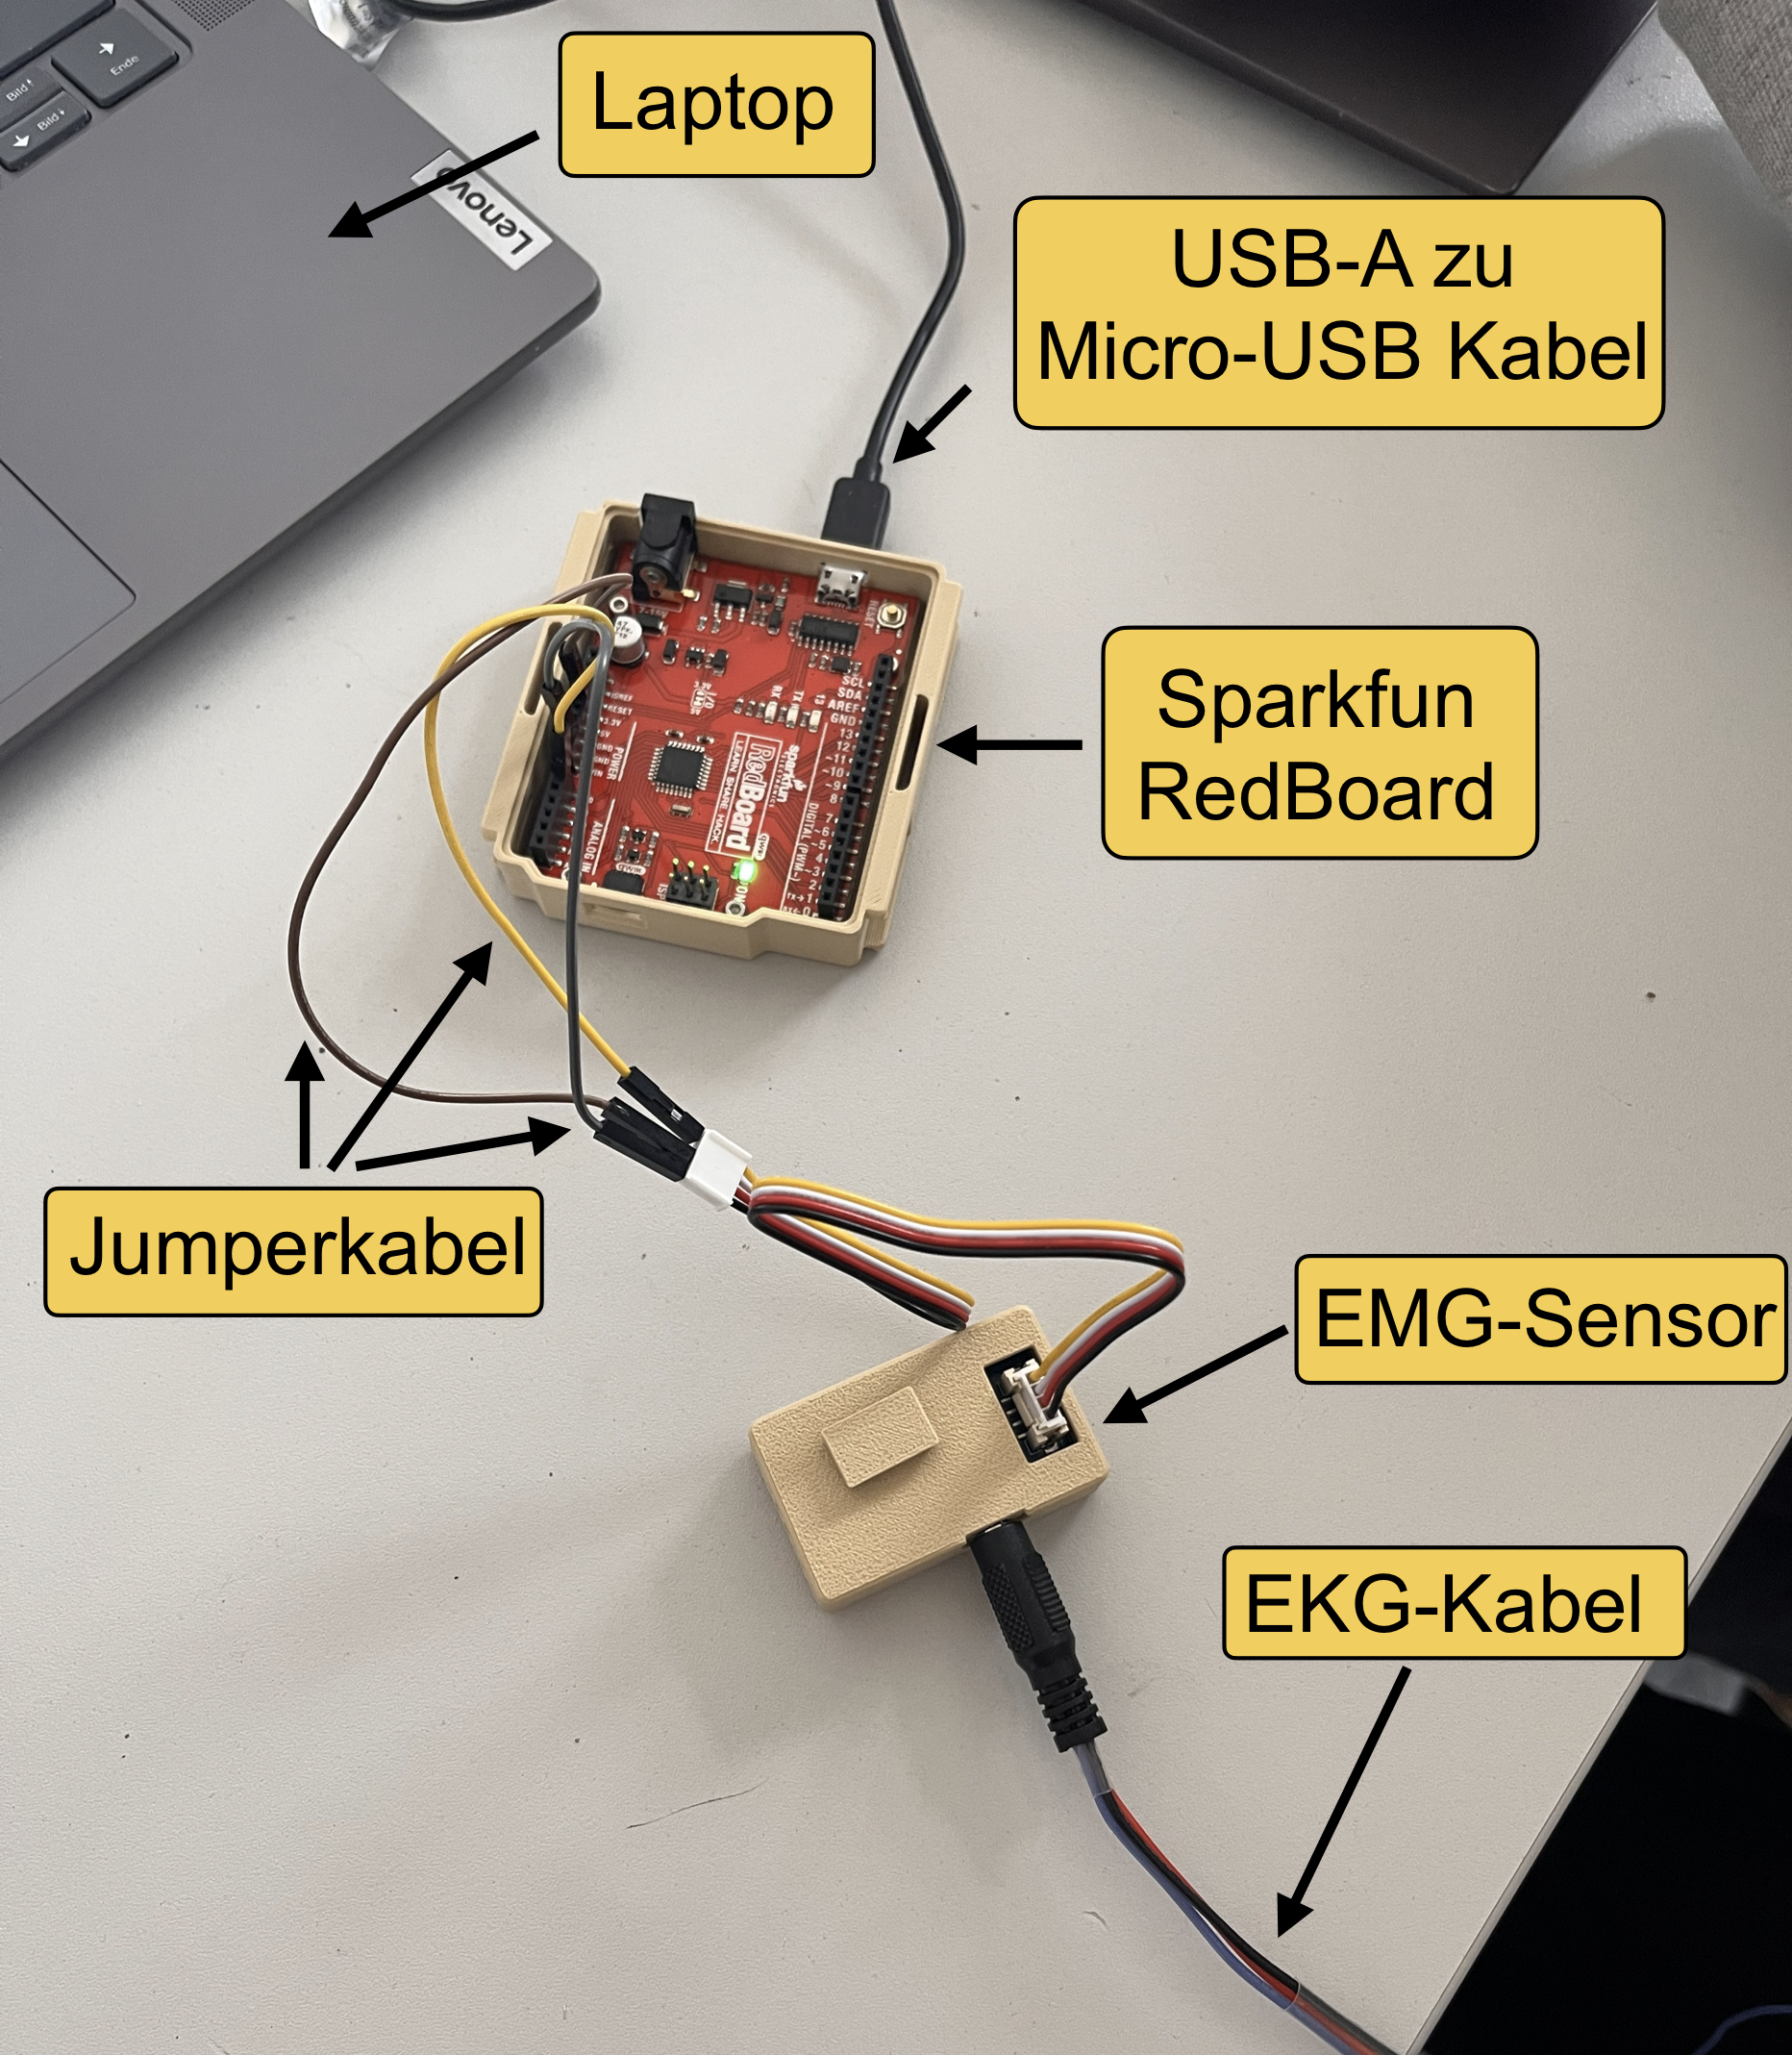
\includegraphics[width=0.4\textwidth]{figures/versuchsaufbau.png}
    \caption{Verbindung des EMG/EKG Sensors mit dem Sparkfun RedBoard Mikrocontroller}
    \label{fig:versuchsaufbau}
\end{figure}

\subsubsection{Platzierung der EKG-Elektroden}
Die Elektroden des Sensors wurden anschließend an den Probanden / die Probanden angebracht. Die drei Elektroden sind am Manubrium, am linken V6 Ableitpunkt und am C7 der Halswirbelsäule angeklebt worden.

\begin{figure}[htbp]
    \centering
    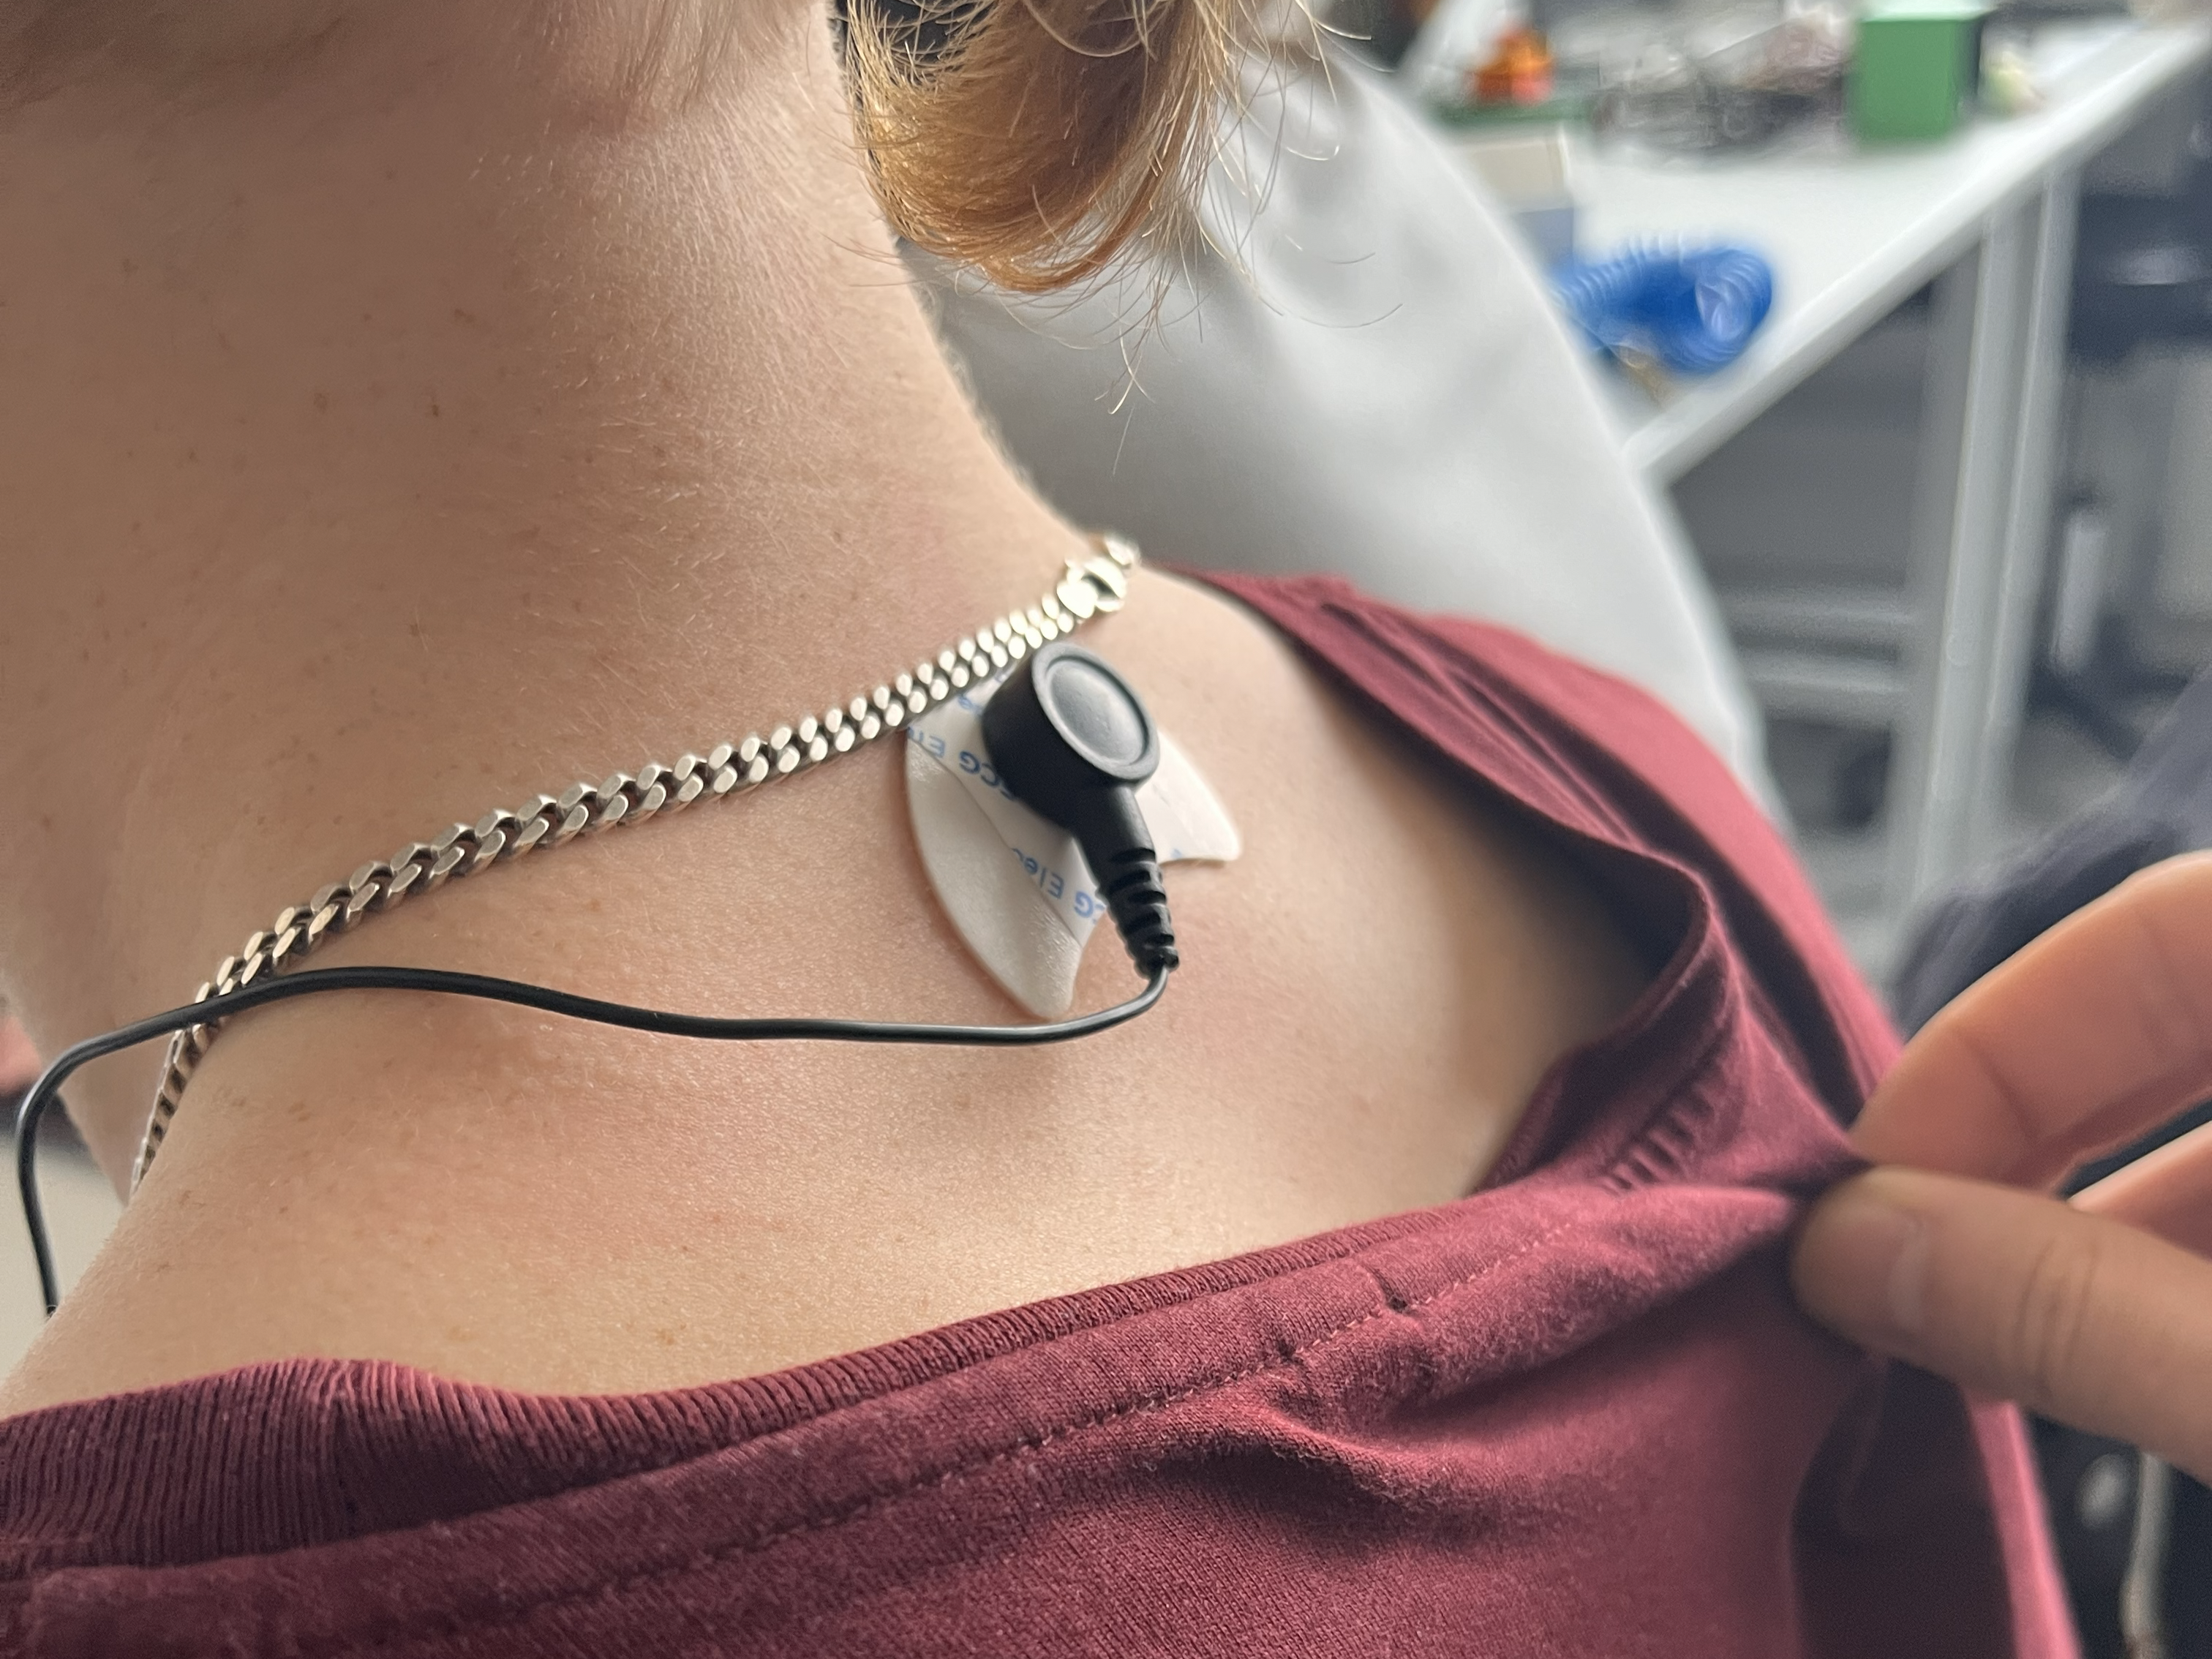
\includegraphics[width=0.4\textwidth]{figures/GNDelectrode_C7.png}
    \caption{Position der Ground-Elektrode auf dem C7 der Halswirbelsäule}
    \label{fig:gnd_electrode_c7}
\end{figure}

In der Abbildung \ref{fig:gnd_electrode_c7} ist die Position der Ground-Elektrode auf dem C7 der Halswirbelsäule zu sehen.

\begin{figure}[htbp]
    \centering
    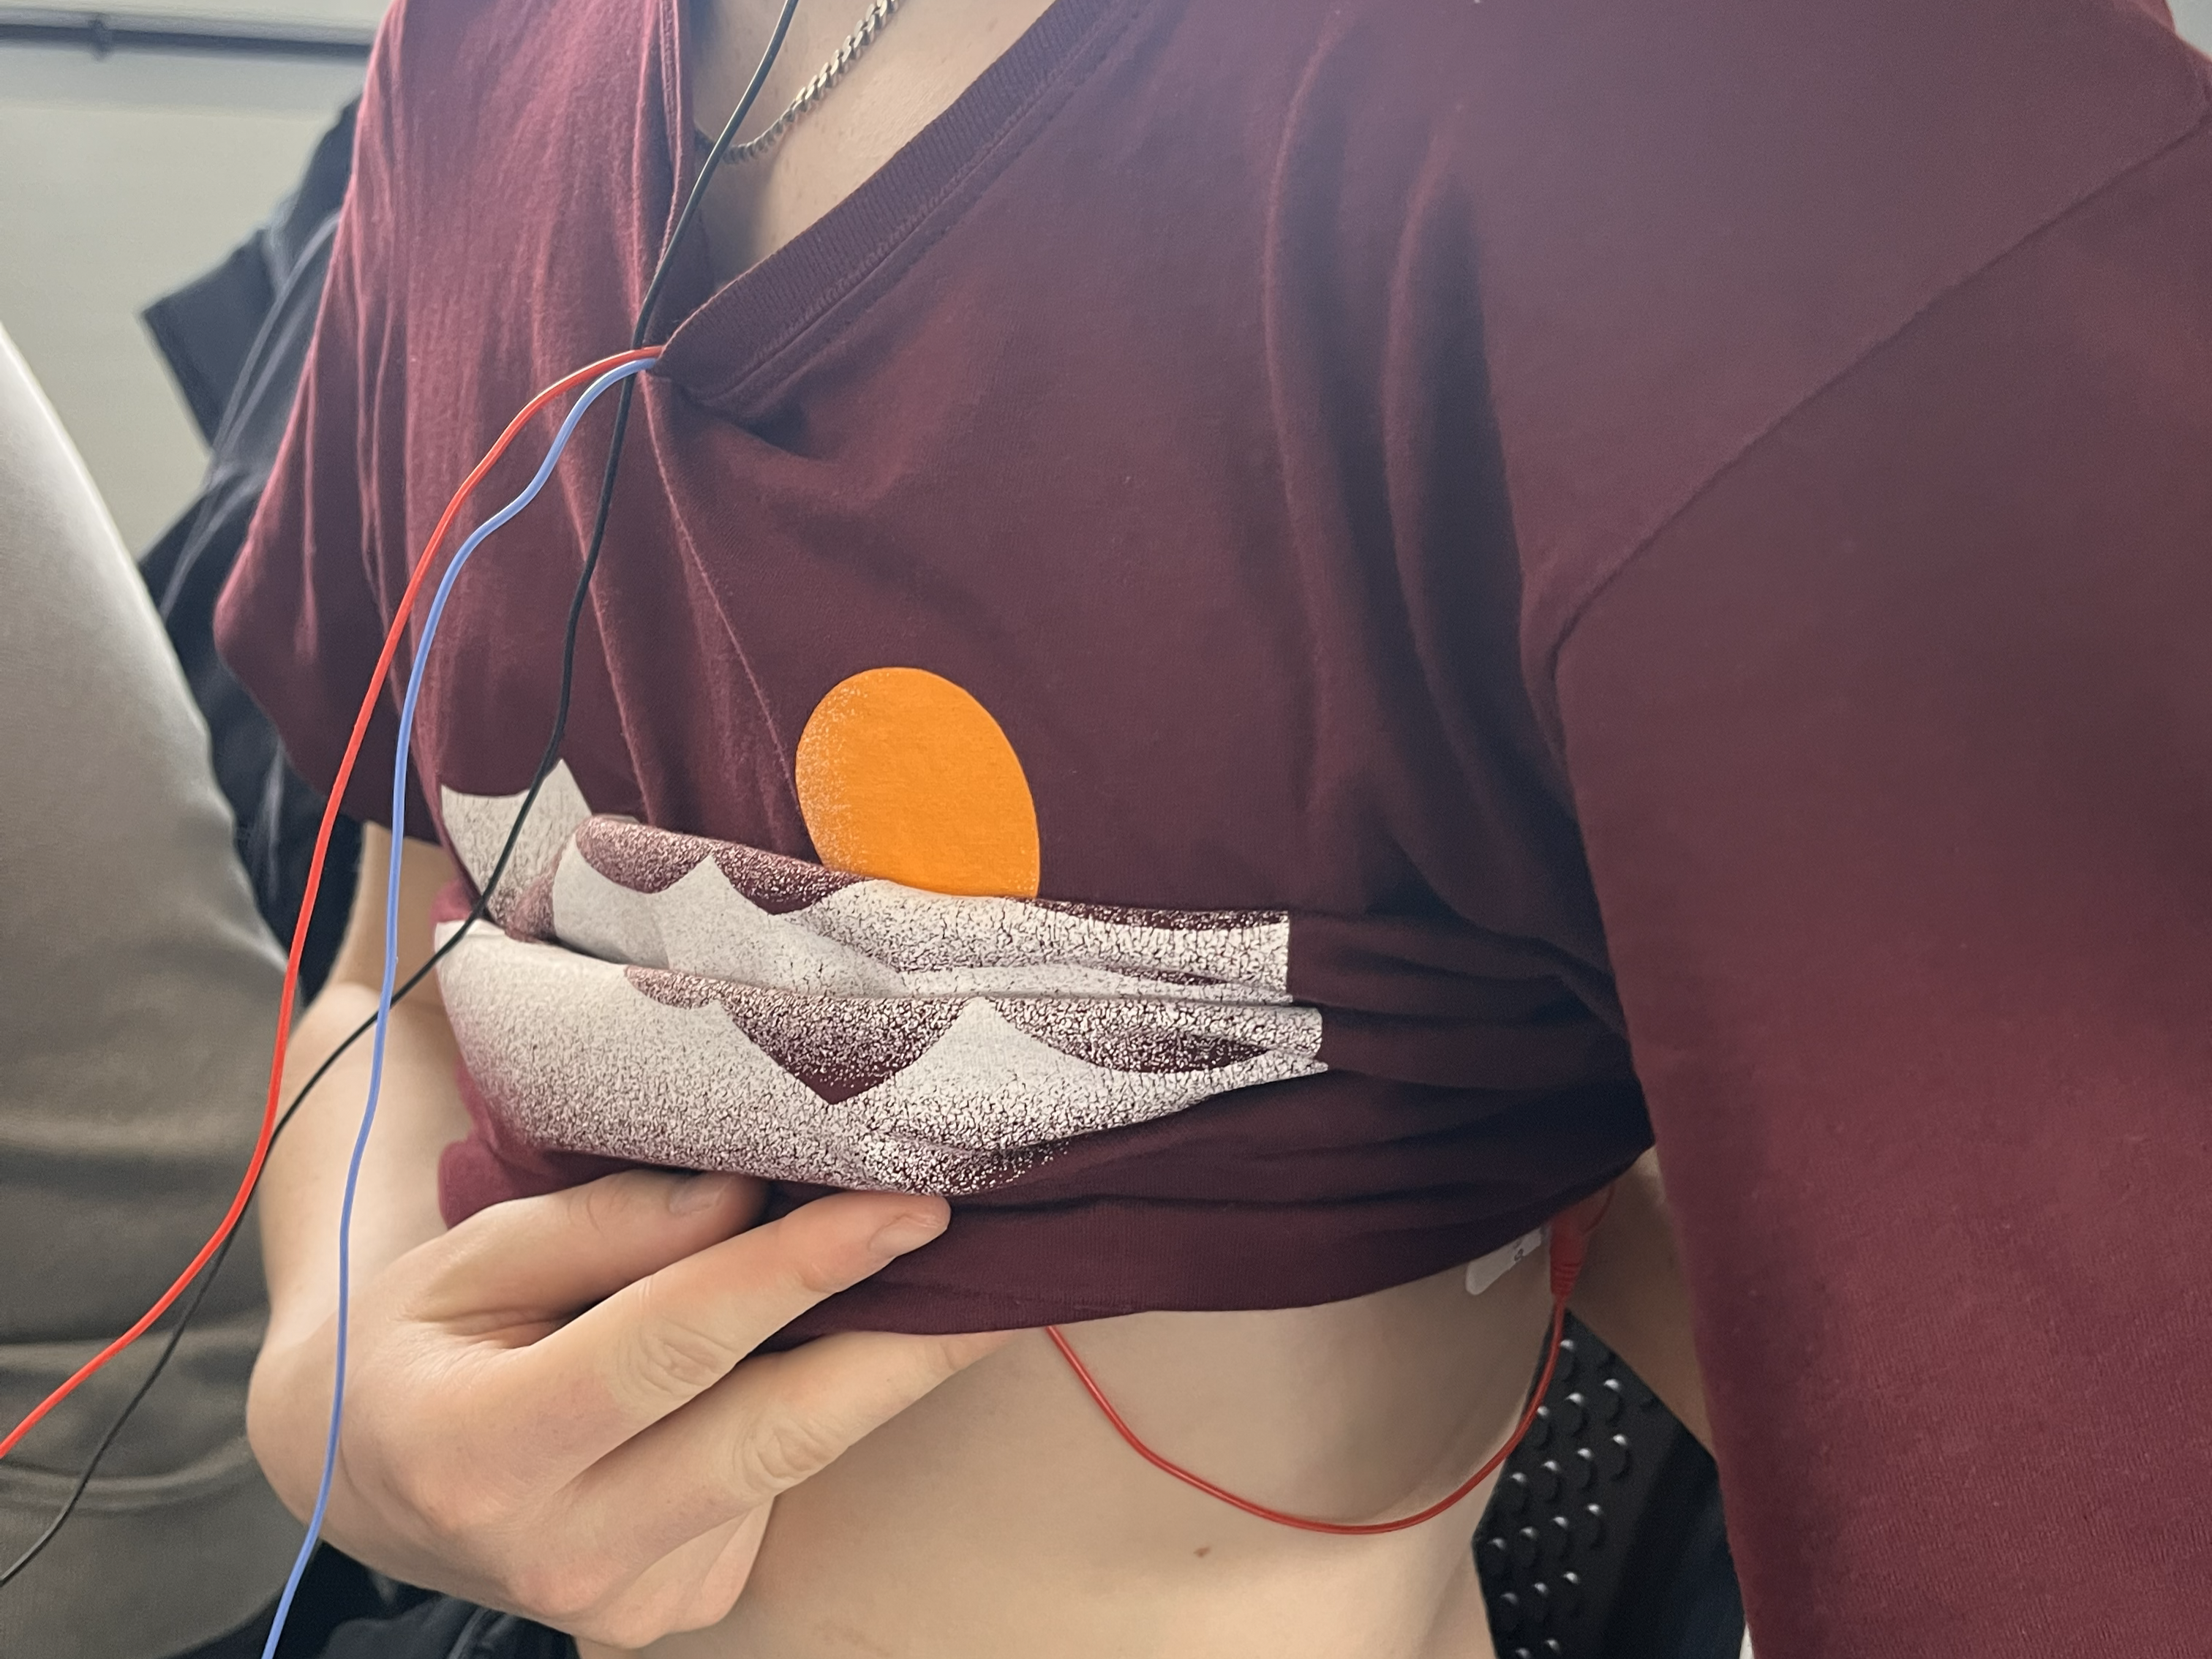
\includegraphics[width=0.4\textwidth]{figures/Manubrium_and_6rip.png}
    \caption{Position der V6-Elektrode auf dem linken V6 Ableitpunkt und der Spannungsquelle auf dem Manubrium}
    \label{fig:v6_electrode_left_and_manubrium}
\end{figure}

In der Abbildung \ref{fig:v6_electrode_left_and_manubrium} ist die Position der V6-Elektrode auf dem linken V6 Ableitpunkt - rotes Kabel - sowie der Spannungsquelle auf dem Manubrium - blaues Kabel - zu sehen.